\documentclass[9pt]{beamer}
\usepackage[utf8]{inputenc}
\usefonttheme{serif} 
\usefonttheme{structuresmallcapsserif} 
\usepackage{hyperref}
\hypersetup{
    colorlinks=true,
    linkcolor=blue,
    filecolor=magenta,
    urlcolor=cyan,
}

\usetheme{Luebeck}
%\usepackage{media9}
%\usepackage{animate}
\usepackage{multimedia}
\usepackage{textpos} 

\addtobeamertemplate{frametitle}{}{%
    \begin{textblock*}{100mm}(11.75cm,-0.86cm)
        
\includegraphics[height=0.86cm,width=0.86cm]{HIPlogo.png}
    \end{textblock*}
    }
\addtobeamertemplate{frametitle}{}{%
    \begin{textblock*}{100mm}(10.89cm,-0.86cm)
        
\includegraphics[height=0.86cm,width=0.86cm]{HYlogo.jpg}
    \end{textblock*}}
\addtobeamertemplate{frametitle}{}{%
    \begin{textblock*}{100mm}(10.03cm,-0.86cm)
        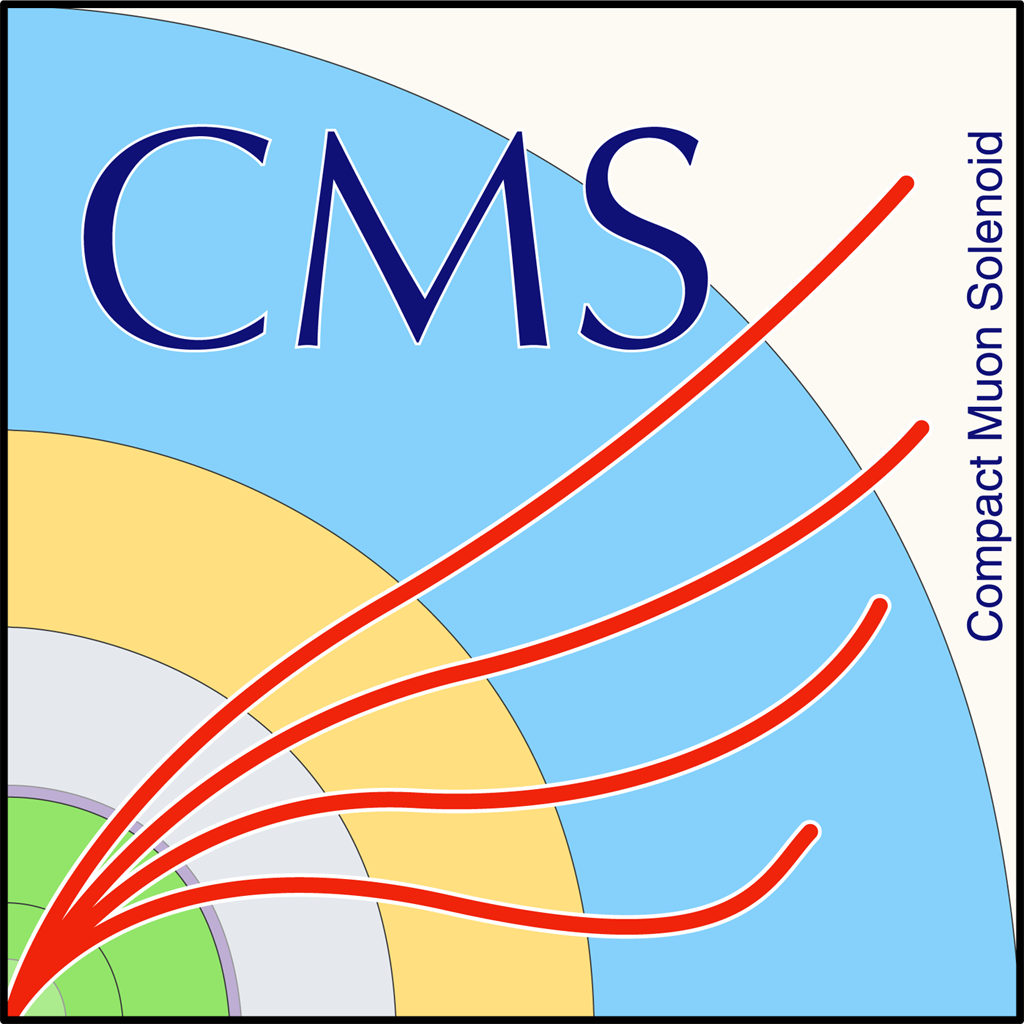
\includegraphics[height=0.86cm,width=0.86cm]{CMSlogo.png}
    \end{textblock*}}

\definecolor{ao}{rgb}{0.0, 0.5, 0.0}
\definecolor{darkgreen}{rgb}{0.0, 0.2, 0.13}
\definecolor{ferngreen}{rgb}{0.31, 0.47, 0.26}
    
\usecolortheme[named=ferngreen]{structure}
\beamertemplatenavigationsymbolsempty
\setbeamertemplate{bibliography item}[text]
\title[ABCD18 (UL ReReco) hot zones]{ABCD18 (UL ReReco) hot zones}
%\subtitle{JERC meeting 26th Feb 2018}
\author{Hannu Siikonen}
\institute{Helsinki Institute of Physics \\ \vspace{0.25cm} Instructor Adj.~Prof.~Mikko~Voutilainen}

\date{\today}

\setbeamersize{text margin left=5pt,text margin right=5pt}
\setlength{\labelsep}{12pt}

\begin{document}

\begin{frame}[t]
\titlepage
\end{frame}

\begin{frame}[t]{Motivation and Practicalities}
\begin{columns}[T]
\begin{column}{\textwidth}
\begin{itemize}
 \item Some parts of the detector might not function optimally
 \item This is seen as an excess (hot zone) or lack (cold zone) of jets
 \item Typically, cold zones are modeled well in MC, but hot zones are not
 \item In precision studies, it makes sense to exclude detector patches that are displayed as such hot zones
 \item The patches for the hot zones are found in the hotjets-*.root file, in the histogram h2hotfilter (also the raw histogram is provided)
 \item In h2hotfilter, a value above zero indicates a hot zone
 \item For simplicity, it can be advisable to use the full-year filter map (which is a sum over all the era filters)
 \item ZeroBias and JetHT samples are used for Data
 \item Standard (flat) QCD + SingleNeutrino samples are used for MC
\end{itemize}
\end{column}
\end{columns}
\end{frame}

\begin{frame}[t]{Methodology and Formulas}
\begin{columns}[T]
\begin{column}{\textwidth}
\begin{itemize}
 \item Fluctuations are studied within bins corresponding to HCAL towers\footnote{Binning picked from L2Relative JEC file}
 \item In one $\eta$ strip of bins, we compute the binwise mean ($\mu$) and sample variance ($s$) of jets passing the jet ID:
 \begin{eqnarray}
     \mu_{\eta}^{trg} &=& \frac{\sum_{i=1}^{N_\phi} N_{jet,\eta}^{i,trg}}{N_\phi} \\
     s_{\eta}^{trg} &=& \sqrt{\frac{\sum_{i=1}^{^{N_\phi}}\left(N_{jet,\eta}^{i,trg}-\mu\right)^2}{N_\phi-1}}
 \end{eqnarray}
 \item The binwise fluctuations are plotted w.r.t. $\sigma$ in the $\eta$ strips with more than 14 of the 72 $\phi$ bins are activated (not empty)
 \item The binwise fluctuations are plotted w.r.t. $\mu$ in the $\eta$ strips where $\mu > \sigma$
 \item We define the following function to help on the next slide
     \begin{equation}
     f(x) =
  \begin{cases}
    0, &\quad\text{if } x < 3\\
    x, &\quad\text{else}
  \end{cases}
 \end{equation}
\end{itemize}
\end{column}
\end{columns}
\end{frame}

\begin{frame}[t]{Calculating the Filter by Trigger Combination}
\begin{columns}[T]
\begin{column}{\textwidth}
\begin{itemize}
 \item Within a single $\eta-\phi$ bin, the $3\sigma+$ fluctuations are summed up from the different triggers (that are usable for the given $|\eta|$ value):
 \begin{equation}
     var_{tot}= \frac{1}{N_{Trg}^{Avail}}\sum_{trg=1}^{N_{Trg}^{Avail}} f\left(\frac{\left(N_{jet,\eta}^{i_\phi,trg} - \mu_\eta^{trg}\right)}{s_\eta^{trg}}\right)
 \end{equation}
    \item The value of $N_{Trg}^{Avail}$ must be determined by looking which triggers provide enough jet statistics up to the current $\eta$ value
    \item Threshold values for $var_{tot}$ to become filter patches are determined as a function of $N_{Trg}^{Avail}$:
        \begin{equation}
            var_{tot}^{thresh} =
     \begin{cases}
       4, &\quad\text{if } N_{Trg}^{Avail} = 1\\
       3, &\quad\text{if } N_{Trg}^{Avail} = 2,3\\
       2, &\quad\text{if } N_{Trg}^{Avail} = 4,5,6\\
       1.5, &\quad\text{if } N_{Trg}^{Avail} = 7,8\\
       1, &\quad\text{else}
     \end{cases}
        \end{equation}
    \item In practice, this means that for a single trigger we require $4\sigma$, for 2 or 3 triggers in average $3\sigma$ per trigger, etc. $\rightarrow$ sensible trigger combination
\end{itemize}
\end{column}
\end{columns}
\end{frame}

\begin{frame}[t]{HLT\_ZeroBias Data}
\begin{columns}[T]
  \begin{column}{.5\textwidth}
  \includegraphics[width=\linewidth]{../pdf/data_DiffPerMean_jt0.pdf}
  \end{column}
  \begin{column}{.5\textwidth}
  \includegraphics[width=\linewidth]{../pdf/data_DiffPerVar_jt0.pdf}
  \end{column}
\end{columns}
\end{frame}

\begin{frame}[t]{HLT\_PFJet40 Data}
\begin{columns}[T]
  \begin{column}{.5\textwidth}
  \includegraphics[width=\linewidth]{../pdf/data_DiffPerMean_jt40.pdf}
  \end{column}
  \begin{column}{.5\textwidth}
  \includegraphics[width=\linewidth]{../pdf/data_DiffPerVar_jt40.pdf}
  \end{column}
\end{columns}
\end{frame}

\begin{frame}[t]{HLT\_PFJet60 Data}
\begin{columns}[T]
  \begin{column}{.5\textwidth}
  \includegraphics[width=\linewidth]{../pdf/data_DiffPerMean_jt60.pdf}
  \end{column}
  \begin{column}{.5\textwidth}
  \includegraphics[width=\linewidth]{../pdf/data_DiffPerVar_jt60.pdf}
  \end{column}
\end{columns}
\end{frame}

\begin{frame}[t]{HLT\_PFJet80 Data}
\begin{columns}[T]
  \begin{column}{.5\textwidth}
  \includegraphics[width=\linewidth]{../pdf/data_DiffPerMean_jt80.pdf}
  \end{column}
  \begin{column}{.5\textwidth}
  \includegraphics[width=\linewidth]{../pdf/data_DiffPerVar_jt80.pdf}
  \end{column}
\end{columns}
\end{frame}

\begin{frame}[t]{HLT\_PFJet140 Data}
\begin{columns}[T]
  \begin{column}{.5\textwidth}
  \includegraphics[width=\linewidth]{../pdf/data_DiffPerMean_jt140.pdf}
  \end{column}
  \begin{column}{.5\textwidth}
  \includegraphics[width=\linewidth]{../pdf/data_DiffPerVar_jt140.pdf}
  \end{column}
\end{columns}
\end{frame}

\begin{frame}[t]{HLT\_PFJet200 Data}
\begin{columns}[T]
  \begin{column}{.5\textwidth}
  \includegraphics[width=\linewidth]{../pdf/data_DiffPerMean_jt200.pdf}
  \end{column}
  \begin{column}{.5\textwidth}
  \includegraphics[width=\linewidth]{../pdf/data_DiffPerVar_jt200.pdf}
  \end{column}
\end{columns}
\end{frame}

\begin{frame}[t]{HLT\_PFJet260 Data}
\begin{columns}[T]
  \begin{column}{.5\textwidth}
  \includegraphics[width=\linewidth]{../pdf/data_DiffPerMean_jt260.pdf}
  \end{column}
  \begin{column}{.5\textwidth}
  \includegraphics[width=\linewidth]{../pdf/data_DiffPerVar_jt260.pdf}
  \end{column}
\end{columns}
\end{frame}

\begin{frame}[t]{HLT\_PFJet320 Data}
\begin{columns}[T]
  \begin{column}{.5\textwidth}
  \includegraphics[width=\linewidth]{../pdf/data_DiffPerMean_jt320.pdf}
  \end{column}
  \begin{column}{.5\textwidth}
  \includegraphics[width=\linewidth]{../pdf/data_DiffPerVar_jt320.pdf}
  \end{column}
\end{columns}
\end{frame}

\begin{frame}[t]{HLT\_PFJet400 Data}
\begin{columns}[T]
  \begin{column}{.5\textwidth}
  \includegraphics[width=\linewidth]{../pdf/data_DiffPerMean_jt400.pdf}
  \end{column}
  \begin{column}{.5\textwidth}
  \includegraphics[width=\linewidth]{../pdf/data_DiffPerVar_jt400.pdf}
  \end{column}
\end{columns}
\end{frame}

\begin{frame}[t]{HLT\_PFJet450 Data}
\begin{columns}[T]
  \begin{column}{.5\textwidth}
  \includegraphics[width=\linewidth]{../pdf/data_DiffPerMean_jt450.pdf}
  \end{column}
  \begin{column}{.5\textwidth}
  \includegraphics[width=\linewidth]{../pdf/data_DiffPerVar_jt450.pdf}
  \end{column}
\end{columns}
\end{frame}

\begin{frame}[t]{HLT\_PFJet500 Data}
\begin{columns}[T]
  \begin{column}{.5\textwidth}
  \includegraphics[width=\linewidth]{../pdf/data_DiffPerMean_jt500.pdf}
  \end{column}
  \begin{column}{.5\textwidth}
  \includegraphics[width=\linewidth]{../pdf/data_DiffPerVar_jt500.pdf}
  \end{column}
\end{columns}
\end{frame}

\begin{frame}[t]{Cumulative summary (P8,DATA)}
\begin{columns}[T]
  \begin{column}{.5\textwidth}
  \includegraphics[width=\linewidth]{../pdf/mc_cumulation.pdf}
  \end{column}
  \begin{column}{.5\textwidth}
  \includegraphics[width=\linewidth]{../pdf/data_cumulation.pdf}
  \end{column}
\end{columns}
\begin{itemize}
 \item Cumulative summary plots over all triggers - attempt to present the excess/deficit plots cumulated over all triggers
 \item In the $\eta$ border zones only the triggers with a sufficient amount of data is used
\end{itemize}
\end{frame}

\begin{frame}[t]{Filtered cumulative summary Data (cold, hot)}
\begin{columns}[T]
  \begin{column}{.5\textwidth}
  \includegraphics[width=\linewidth]{../pdf/data_colds.pdf}
  \end{column}
  \begin{column}{.5\textwidth}
  \includegraphics[width=\linewidth]{../pdf/data_hots.pdf}
  \end{column}
\end{columns}
\begin{itemize}
 \item The same procedure as on the previous slide, but now we emphasize noise that is significant in more than only one trigger
 \item Hot and cold zones separated
\end{itemize}
\end{frame}

\begin{frame}[t]{Filtered cumulative summary P8 (cold, hot)}
\begin{columns}[T]
  \begin{column}{.5\textwidth}
  \includegraphics[width=\linewidth]{../pdf/mc_colds.pdf}
  \end{column}
  \begin{column}{.5\textwidth}
  \includegraphics[width=\linewidth]{../pdf/mc_hots.pdf}
  \end{column}
\end{columns}
\begin{itemize}
 \item The same procedure as on the previous slide, but now we emphasize noise that is significant in more than only one trigger
 \item Hot and cold zones separated
\end{itemize}
\end{frame}

\begin{frame}[t]{Jet counts ZeroBias (P8,DATA)}
\begin{columns}[T]
  \begin{column}{.5\textwidth}
  \includegraphics[width=\linewidth]{../pdf/mc_njet_jt0.pdf}
  \end{column}
  \begin{column}{.5\textwidth}
  \includegraphics[width=\linewidth]{../pdf/data_njet_jt0.pdf}
  \end{column}
\end{columns}
\begin{itemize}
 \item Left: Pythia~8; Right: Data
 \item White patches: $3\sigma+$ downwards fluctuations for this trigger
 \item Black patches: $3\sigma+$ upwards fluctuations for this trigger
\end{itemize}
\end{frame}

\begin{frame}[t]{Jet counts JetHT40 (P8,DATA)}
\begin{columns}[T]
  \begin{column}{.5\textwidth}
  \includegraphics[width=\linewidth]{../pdf/mc_njet_jt40.pdf}
  \end{column}
  \begin{column}{.5\textwidth}
  \includegraphics[width=\linewidth]{../pdf/data_njet_jt40.pdf}
  \end{column}
\end{columns}
\begin{itemize}
 \item Left: Pythia~8; Right: Data
 \item White patches: $3\sigma+$ downwards fluctuations for this trigger
 \item Black patches: $3\sigma+$ upwards fluctuations for this trigger
\end{itemize}
\end{frame}

\begin{frame}[t]{Jet counts JetHT60 (P8,DATA)}
\begin{columns}[T]
  \begin{column}{.5\textwidth}
  \includegraphics[width=\linewidth]{../pdf/mc_njet_jt60.pdf}
  \end{column}
  \begin{column}{.5\textwidth}
  \includegraphics[width=\linewidth]{../pdf/data_njet_jt60.pdf}
  \end{column}
\end{columns}
\begin{itemize}
 \item Left: Pythia~8; Right: Data
 \item White patches: $3\sigma+$ downwards fluctuations for this trigger
 \item Black patches: $3\sigma+$ upwards fluctuations for this trigger
\end{itemize}
\end{frame}

\begin{frame}[t]{Jet counts JetHT80 (P8,DATA)}
\begin{columns}[T]
  \begin{column}{.5\textwidth}
  \includegraphics[width=\linewidth]{../pdf/mc_njet_jt80.pdf}
  \end{column}
  \begin{column}{.5\textwidth}
  \includegraphics[width=\linewidth]{../pdf/data_njet_jt80.pdf}
  \end{column}
\end{columns}
\begin{itemize}
 \item Left: Pythia~8; Right: Data
 \item White patches: $3\sigma+$ downwards fluctuations for this trigger
 \item Black patches: $3\sigma+$ upwards fluctuations for this trigger
\end{itemize}
\end{frame}

\begin{frame}[t]{Jet counts JetHT140 (P8,DATA)}
\begin{columns}[T]
  \begin{column}{.5\textwidth}
  \includegraphics[width=\linewidth]{../pdf/mc_njet_jt140.pdf}
  \end{column}
  \begin{column}{.5\textwidth}
  \includegraphics[width=\linewidth]{../pdf/data_njet_jt140.pdf}
  \end{column}
\end{columns}
\begin{itemize}
 \item Left: Pythia~8; Right: Data
 \item White patches: $3\sigma+$ downwards fluctuations for this trigger
 \item Black patches: $3\sigma+$ upwards fluctuations for this trigger
\end{itemize}
\end{frame}

\begin{frame}[t]{Jet counts JetHT200 (P8,DATA)}
\begin{columns}[T]
  \begin{column}{.5\textwidth}
  \includegraphics[width=\linewidth]{../pdf/mc_njet_jt200.pdf}
  \end{column}
  \begin{column}{.5\textwidth}
  \includegraphics[width=\linewidth]{../pdf/data_njet_jt200.pdf}
  \end{column}
\end{columns}
\begin{itemize}
 \item Left: Pythia~8; Right: Data
 \item White patches: $3\sigma+$ downwards fluctuations for this trigger
 \item Black patches: $3\sigma+$ upwards fluctuations for this trigger
\end{itemize}
\end{frame}

\begin{frame}[t]{Jet counts JetHT260 (P8,DATA)}
\begin{columns}[T]
  \begin{column}{.5\textwidth}
  \includegraphics[width=\linewidth]{../pdf/mc_njet_jt260.pdf}
  \end{column}
  \begin{column}{.5\textwidth}
  \includegraphics[width=\linewidth]{../pdf/data_njet_jt260.pdf}
  \end{column}
\end{columns}
\begin{itemize}
 \item Left: Pythia~8; Right: Data
 \item White patches: $3\sigma+$ downwards fluctuations for this trigger
 \item Black patches: $3\sigma+$ upwards fluctuations for this trigger
\end{itemize}
\end{frame}

\begin{frame}[t]{Jet counts JetHT320 (P8,DATA)}
\begin{columns}[T]
  \begin{column}{.5\textwidth}
  \includegraphics[width=\linewidth]{../pdf/mc_njet_jt320.pdf}
  \end{column}
  \begin{column}{.5\textwidth}
  \includegraphics[width=\linewidth]{../pdf/data_njet_jt320.pdf}
  \end{column}
\end{columns}
\begin{itemize}
 \item Left: Pythia~8; Right: Data
 \item White patches: $3\sigma+$ downwards fluctuations for this trigger
 \item Black patches: $3\sigma+$ upwards fluctuations for this trigger
\end{itemize}
\end{frame}

\begin{frame}[t]{Jet counts JetHT400 (P8,DATA)}
\begin{columns}[T]
  \begin{column}{.5\textwidth}
  \includegraphics[width=\linewidth]{../pdf/mc_njet_jt400.pdf}
  \end{column}
  \begin{column}{.5\textwidth}
  \includegraphics[width=\linewidth]{../pdf/data_njet_jt400.pdf}
  \end{column}
\end{columns}
\begin{itemize}
 \item Left: Pythia~8; Right: Data
 \item White patches: $3\sigma+$ downwards fluctuations for this trigger
 \item Black patches: $3\sigma+$ upwards fluctuations for this trigger
\end{itemize}
\end{frame}

\begin{frame}[t]{Jet counts JetHT450 (P8,DATA)}
\begin{columns}[T]
  \begin{column}{.5\textwidth}
  \includegraphics[width=\linewidth]{../pdf/mc_njet_jt450.pdf}
  \end{column}
  \begin{column}{.5\textwidth}
  \includegraphics[width=\linewidth]{../pdf/data_njet_jt450.pdf}
  \end{column}
\end{columns}
\begin{itemize}
 \item Left: Pythia~8; Right: Data
 \item White patches: $3\sigma+$ downwards fluctuations for this trigger
 \item Black patches: $3\sigma+$ upwards fluctuations for this trigger
\end{itemize}
\end{frame}

\begin{frame}[t]{Jet counts JetHT500 (P8,DATA)}
\begin{columns}[T]
  \begin{column}{.5\textwidth}
  \includegraphics[width=\linewidth]{../pdf/mc_njet_jt500.pdf}
  \end{column}
  \begin{column}{.5\textwidth}
  \includegraphics[width=\linewidth]{../pdf/data_njet_jt500.pdf}
  \end{column}
\end{columns}
\begin{itemize}
 \item Left: Pythia~8; Right: Data
 \item White patches: $3\sigma+$ downwards fluctuations for this trigger
 \item Black patches: $3\sigma+$ upwards fluctuations for this trigger
\end{itemize}
\end{frame}


\begin{frame}[t]{HLT\_ZeroBias Data chf}
\begin{columns}[T]
  \begin{column}{.5\textwidth}
  \includegraphics[width=\linewidth]{../pdf/data_DiffPerMean_chf_jt0.pdf}
  \end{column}
  \begin{column}{.5\textwidth}
  \includegraphics[width=\linewidth]{../pdf/data_DiffPerVar_chf_jt0.pdf}
  \end{column}
\end{columns}
\end{frame}

\begin{frame}[t]{HLT\_PFJet40 Data chf}
\begin{columns}[T]
  \begin{column}{.5\textwidth}
  \includegraphics[width=\linewidth]{../pdf/data_DiffPerMean_chf_jt40.pdf}
  \end{column}
  \begin{column}{.5\textwidth}
  \includegraphics[width=\linewidth]{../pdf/data_DiffPerVar_chf_jt40.pdf}
  \end{column}
\end{columns}
\end{frame}

\begin{frame}[t]{HLT\_PFJet60 Data chf}
\begin{columns}[T]
  \begin{column}{.5\textwidth}
  \includegraphics[width=\linewidth]{../pdf/data_DiffPerMean_chf_jt60.pdf}
  \end{column}
  \begin{column}{.5\textwidth}
  \includegraphics[width=\linewidth]{../pdf/data_DiffPerVar_chf_jt60.pdf}
  \end{column}
\end{columns}
\end{frame}

\begin{frame}[t]{HLT\_PFJet80 Data chf}
\begin{columns}[T]
  \begin{column}{.5\textwidth}
  \includegraphics[width=\linewidth]{../pdf/data_DiffPerMean_chf_jt80.pdf}
  \end{column}
  \begin{column}{.5\textwidth}
  \includegraphics[width=\linewidth]{../pdf/data_DiffPerVar_chf_jt80.pdf}
  \end{column}
\end{columns}
\end{frame}

\begin{frame}[t]{HLT\_PFJet140 Data chf}
\begin{columns}[T]
  \begin{column}{.5\textwidth}
  \includegraphics[width=\linewidth]{../pdf/data_DiffPerMean_chf_jt140.pdf}
  \end{column}
  \begin{column}{.5\textwidth}
  \includegraphics[width=\linewidth]{../pdf/data_DiffPerVar_chf_jt140.pdf}
  \end{column}
\end{columns}
\end{frame}

\begin{frame}[t]{HLT\_PFJet200 Data chf}
\begin{columns}[T]
  \begin{column}{.5\textwidth}
  \includegraphics[width=\linewidth]{../pdf/data_DiffPerMean_chf_jt200.pdf}
  \end{column}
  \begin{column}{.5\textwidth}
  \includegraphics[width=\linewidth]{../pdf/data_DiffPerVar_chf_jt200.pdf}
  \end{column}
\end{columns}
\end{frame}

\begin{frame}[t]{HLT\_PFJet260 Data chf}
\begin{columns}[T]
  \begin{column}{.5\textwidth}
  \includegraphics[width=\linewidth]{../pdf/data_DiffPerMean_chf_jt260.pdf}
  \end{column}
  \begin{column}{.5\textwidth}
  \includegraphics[width=\linewidth]{../pdf/data_DiffPerVar_chf_jt260.pdf}
  \end{column}
\end{columns}
\end{frame}

\begin{frame}[t]{HLT\_PFJet320 Data chf}
\begin{columns}[T]
  \begin{column}{.5\textwidth}
  \includegraphics[width=\linewidth]{../pdf/data_DiffPerMean_chf_jt320.pdf}
  \end{column}
  \begin{column}{.5\textwidth}
  \includegraphics[width=\linewidth]{../pdf/data_DiffPerVar_chf_jt320.pdf}
  \end{column}
\end{columns}
\end{frame}

\begin{frame}[t]{HLT\_PFJet400 Data chf}
\begin{columns}[T]
  \begin{column}{.5\textwidth}
  \includegraphics[width=\linewidth]{../pdf/data_DiffPerMean_chf_jt400.pdf}
  \end{column}
  \begin{column}{.5\textwidth}
  \includegraphics[width=\linewidth]{../pdf/data_DiffPerVar_chf_jt400.pdf}
  \end{column}
\end{columns}
\end{frame}

\begin{frame}[t]{HLT\_PFJet450 Data chf}
\begin{columns}[T]
  \begin{column}{.5\textwidth}
  \includegraphics[width=\linewidth]{../pdf/data_DiffPerMean_chf_jt450.pdf}
  \end{column}
  \begin{column}{.5\textwidth}
  \includegraphics[width=\linewidth]{../pdf/data_DiffPerVar_chf_jt450.pdf}
  \end{column}
\end{columns}
\end{frame}

\begin{frame}[t]{HLT\_PFJet500 Data chf}
\begin{columns}[T]
  \begin{column}{.5\textwidth}
  \includegraphics[width=\linewidth]{../pdf/data_DiffPerMean_chf_jt500.pdf}
  \end{column}
  \begin{column}{.5\textwidth}
  \includegraphics[width=\linewidth]{../pdf/data_DiffPerVar_chf_jt500.pdf}
  \end{column}
\end{columns}
\end{frame}

\begin{frame}[t]{Cumulative summary (P8,DATA)}
\begin{columns}[T]
  \begin{column}{.5\textwidth}
  \includegraphics[width=\linewidth]{../pdf/mc_chf_cumulation.pdf}
  \end{column}
  \begin{column}{.5\textwidth}
  \includegraphics[width=\linewidth]{../pdf/data_chf_cumulation.pdf}
  \end{column}
\end{columns}
\begin{itemize}
 \item Cumulative summary plots over all triggers - attempt to present the excess/deficit plots cumulated over all triggers
 \item In the $\eta$ border zones only the triggers with a sufficient amount of data is used
\end{itemize}
\end{frame}

\begin{frame}[t]{Filtered cumulative summary Data chf (cold, hot)}
\begin{columns}[T]
  \begin{column}{.5\textwidth}
  \includegraphics[width=\linewidth]{../pdf/data_chf_colds.pdf}
  \end{column}
  \begin{column}{.5\textwidth}
  \includegraphics[width=\linewidth]{../pdf/data_chf_hots.pdf}
  \end{column}
\end{columns}
\begin{itemize}
 \item The same procedure as on the previous slide, but now we emphasize noise that is significant in more than only one trigger
 \item Hot and cold zones separated
\end{itemize}
\end{frame}

\begin{frame}[t]{Filtered cumulative summary P8 (cold, hot)}
\begin{columns}[T]
  \begin{column}{.5\textwidth}
  \includegraphics[width=\linewidth]{../pdf/mc_chf_colds.pdf}
  \end{column}
  \begin{column}{.5\textwidth}
  \includegraphics[width=\linewidth]{../pdf/mc_chf_hots.pdf}
  \end{column}
\end{columns}
\begin{itemize}
 \item The same procedure as on the previous slide, but now we emphasize noise that is significant in more than only one trigger
 \item Hot and cold zones separated
\end{itemize}
\end{frame}


\begin{frame}[t]{HLT\_ZeroBias Data puf}
\begin{columns}[T]
  \begin{column}{.5\textwidth}
  \includegraphics[width=\linewidth]{../pdf/data_DiffPerMean_puf_jt0.pdf}
  \end{column}
  \begin{column}{.5\textwidth}
  \includegraphics[width=\linewidth]{../pdf/data_DiffPerVar_puf_jt0.pdf}
  \end{column}
\end{columns}
\end{frame}

\begin{frame}[t]{HLT\_PFJet40 Data puf}
\begin{columns}[T]
  \begin{column}{.5\textwidth}
  \includegraphics[width=\linewidth]{../pdf/data_DiffPerMean_puf_jt40.pdf}
  \end{column}
  \begin{column}{.5\textwidth}
  \includegraphics[width=\linewidth]{../pdf/data_DiffPerVar_puf_jt40.pdf}
  \end{column}
\end{columns}
\end{frame}

\begin{frame}[t]{HLT\_PFJet60 Data puf}
\begin{columns}[T]
  \begin{column}{.5\textwidth}
  \includegraphics[width=\linewidth]{../pdf/data_DiffPerMean_puf_jt60.pdf}
  \end{column}
  \begin{column}{.5\textwidth}
  \includegraphics[width=\linewidth]{../pdf/data_DiffPerVar_puf_jt60.pdf}
  \end{column}
\end{columns}
\end{frame}

\begin{frame}[t]{HLT\_PFJet80 Data puf}
\begin{columns}[T]
  \begin{column}{.5\textwidth}
  \includegraphics[width=\linewidth]{../pdf/data_DiffPerMean_puf_jt80.pdf}
  \end{column}
  \begin{column}{.5\textwidth}
  \includegraphics[width=\linewidth]{../pdf/data_DiffPerVar_puf_jt80.pdf}
  \end{column}
\end{columns}
\end{frame}

\begin{frame}[t]{HLT\_PFJet140 Data puf}
\begin{columns}[T]
  \begin{column}{.5\textwidth}
  \includegraphics[width=\linewidth]{../pdf/data_DiffPerMean_puf_jt140.pdf}
  \end{column}
  \begin{column}{.5\textwidth}
  \includegraphics[width=\linewidth]{../pdf/data_DiffPerVar_puf_jt140.pdf}
  \end{column}
\end{columns}
\end{frame}

\begin{frame}[t]{HLT\_PFJet200 Data puf}
\begin{columns}[T]
  \begin{column}{.5\textwidth}
  \includegraphics[width=\linewidth]{../pdf/data_DiffPerMean_puf_jt200.pdf}
  \end{column}
  \begin{column}{.5\textwidth}
  \includegraphics[width=\linewidth]{../pdf/data_DiffPerVar_puf_jt200.pdf}
  \end{column}
\end{columns}
\end{frame}

\begin{frame}[t]{HLT\_PFJet260 Data puf}
\begin{columns}[T]
  \begin{column}{.5\textwidth}
  \includegraphics[width=\linewidth]{../pdf/data_DiffPerMean_puf_jt260.pdf}
  \end{column}
  \begin{column}{.5\textwidth}
  \includegraphics[width=\linewidth]{../pdf/data_DiffPerVar_puf_jt260.pdf}
  \end{column}
\end{columns}
\end{frame}

\begin{frame}[t]{HLT\_PFJet320 Data puf}
\begin{columns}[T]
  \begin{column}{.5\textwidth}
  \includegraphics[width=\linewidth]{../pdf/data_DiffPerMean_puf_jt320.pdf}
  \end{column}
  \begin{column}{.5\textwidth}
  \includegraphics[width=\linewidth]{../pdf/data_DiffPerVar_puf_jt320.pdf}
  \end{column}
\end{columns}
\end{frame}

\begin{frame}[t]{HLT\_PFJet400 Data puf}
\begin{columns}[T]
  \begin{column}{.5\textwidth}
  \includegraphics[width=\linewidth]{../pdf/data_DiffPerMean_puf_jt400.pdf}
  \end{column}
  \begin{column}{.5\textwidth}
  \includegraphics[width=\linewidth]{../pdf/data_DiffPerVar_puf_jt400.pdf}
  \end{column}
\end{columns}
\end{frame}

\begin{frame}[t]{HLT\_PFJet450 Data puf}
\begin{columns}[T]
  \begin{column}{.5\textwidth}
  \includegraphics[width=\linewidth]{../pdf/data_DiffPerMean_puf_jt450.pdf}
  \end{column}
  \begin{column}{.5\textwidth}
  \includegraphics[width=\linewidth]{../pdf/data_DiffPerVar_puf_jt450.pdf}
  \end{column}
\end{columns}
\end{frame}

\begin{frame}[t]{HLT\_PFJet500 Data puf}
\begin{columns}[T]
  \begin{column}{.5\textwidth}
  \includegraphics[width=\linewidth]{../pdf/data_DiffPerMean_puf_jt500.pdf}
  \end{column}
  \begin{column}{.5\textwidth}
  \includegraphics[width=\linewidth]{../pdf/data_DiffPerVar_puf_jt500.pdf}
  \end{column}
\end{columns}
\end{frame}

\begin{frame}[t]{Cumulative summary (P8,DATA)}
\begin{columns}[T]
  \begin{column}{.5\textwidth}
  \includegraphics[width=\linewidth]{../pdf/mc_puf_cumulation.pdf}
  \end{column}
  \begin{column}{.5\textwidth}
  \includegraphics[width=\linewidth]{../pdf/data_puf_cumulation.pdf}
  \end{column}
\end{columns}
\begin{itemize}
 \item Cumulative summary plots over all triggers - attempt to present the excess/deficit plots cumulated over all triggers
 \item In the $\eta$ border zones only the triggers with a sufficient amount of data is used
\end{itemize}
\end{frame}

\begin{frame}[t]{Filtered cumulative summary Data puf (cold, hot)}
\begin{columns}[T]
  \begin{column}{.5\textwidth}
  \includegraphics[width=\linewidth]{../pdf/data_puf_colds.pdf}
  \end{column}
  \begin{column}{.5\textwidth}
  \includegraphics[width=\linewidth]{../pdf/data_puf_hots.pdf}
  \end{column}
\end{columns}
\begin{itemize}
 \item The same procedure as on the previous slide, but now we emphasize noise that is significant in more than only one trigger
 \item Hot and cold zones separated
\end{itemize}
\end{frame}

\begin{frame}[t]{Filtered cumulative summary P8 (cold, hot)}
\begin{columns}[T]
  \begin{column}{.5\textwidth}
  \includegraphics[width=\linewidth]{../pdf/mc_puf_colds.pdf}
  \end{column}
  \begin{column}{.5\textwidth}
  \includegraphics[width=\linewidth]{../pdf/mc_puf_hots.pdf}
  \end{column}
\end{columns}
\begin{itemize}
 \item The same procedure as on the previous slide, but now we emphasize noise that is significant in more than only one trigger
 \item Hot and cold zones separated
\end{itemize}
\end{frame}


\begin{frame}[t]{HLT\_ZeroBias Data nhf}
\begin{columns}[T]
  \begin{column}{.5\textwidth}
  \includegraphics[width=\linewidth]{../pdf/data_DiffPerMean_nhf_jt0.pdf}
  \end{column}
  \begin{column}{.5\textwidth}
  \includegraphics[width=\linewidth]{../pdf/data_DiffPerVar_nhf_jt0.pdf}
  \end{column}
\end{columns}
\end{frame}

\begin{frame}[t]{HLT\_PFJet40 Data nhf}
\begin{columns}[T]
  \begin{column}{.5\textwidth}
  \includegraphics[width=\linewidth]{../pdf/data_DiffPerMean_nhf_jt40.pdf}
  \end{column}
  \begin{column}{.5\textwidth}
  \includegraphics[width=\linewidth]{../pdf/data_DiffPerVar_nhf_jt40.pdf}
  \end{column}
\end{columns}
\end{frame}

\begin{frame}[t]{HLT\_PFJet60 Data nhf}
\begin{columns}[T]
  \begin{column}{.5\textwidth}
  \includegraphics[width=\linewidth]{../pdf/data_DiffPerMean_nhf_jt60.pdf}
  \end{column}
  \begin{column}{.5\textwidth}
  \includegraphics[width=\linewidth]{../pdf/data_DiffPerVar_nhf_jt60.pdf}
  \end{column}
\end{columns}
\end{frame}

\begin{frame}[t]{HLT\_PFJet80 Data nhf}
\begin{columns}[T]
  \begin{column}{.5\textwidth}
  \includegraphics[width=\linewidth]{../pdf/data_DiffPerMean_nhf_jt80.pdf}
  \end{column}
  \begin{column}{.5\textwidth}
  \includegraphics[width=\linewidth]{../pdf/data_DiffPerVar_nhf_jt80.pdf}
  \end{column}
\end{columns}
\end{frame}

\begin{frame}[t]{HLT\_PFJet140 Data nhf}
\begin{columns}[T]
  \begin{column}{.5\textwidth}
  \includegraphics[width=\linewidth]{../pdf/data_DiffPerMean_nhf_jt140.pdf}
  \end{column}
  \begin{column}{.5\textwidth}
  \includegraphics[width=\linewidth]{../pdf/data_DiffPerVar_nhf_jt140.pdf}
  \end{column}
\end{columns}
\end{frame}

\begin{frame}[t]{HLT\_PFJet200 Data nhf}
\begin{columns}[T]
  \begin{column}{.5\textwidth}
  \includegraphics[width=\linewidth]{../pdf/data_DiffPerMean_nhf_jt200.pdf}
  \end{column}
  \begin{column}{.5\textwidth}
  \includegraphics[width=\linewidth]{../pdf/data_DiffPerVar_nhf_jt200.pdf}
  \end{column}
\end{columns}
\end{frame}

\begin{frame}[t]{HLT\_PFJet260 Data nhf}
\begin{columns}[T]
  \begin{column}{.5\textwidth}
  \includegraphics[width=\linewidth]{../pdf/data_DiffPerMean_nhf_jt260.pdf}
  \end{column}
  \begin{column}{.5\textwidth}
  \includegraphics[width=\linewidth]{../pdf/data_DiffPerVar_nhf_jt260.pdf}
  \end{column}
\end{columns}
\end{frame}

\begin{frame}[t]{HLT\_PFJet320 Data nhf}
\begin{columns}[T]
  \begin{column}{.5\textwidth}
  \includegraphics[width=\linewidth]{../pdf/data_DiffPerMean_nhf_jt320.pdf}
  \end{column}
  \begin{column}{.5\textwidth}
  \includegraphics[width=\linewidth]{../pdf/data_DiffPerVar_nhf_jt320.pdf}
  \end{column}
\end{columns}
\end{frame}

\begin{frame}[t]{HLT\_PFJet400 Data nhf}
\begin{columns}[T]
  \begin{column}{.5\textwidth}
  \includegraphics[width=\linewidth]{../pdf/data_DiffPerMean_nhf_jt400.pdf}
  \end{column}
  \begin{column}{.5\textwidth}
  \includegraphics[width=\linewidth]{../pdf/data_DiffPerVar_nhf_jt400.pdf}
  \end{column}
\end{columns}
\end{frame}

\begin{frame}[t]{HLT\_PFJet450 Data nhf}
\begin{columns}[T]
  \begin{column}{.5\textwidth}
  \includegraphics[width=\linewidth]{../pdf/data_DiffPerMean_nhf_jt450.pdf}
  \end{column}
  \begin{column}{.5\textwidth}
  \includegraphics[width=\linewidth]{../pdf/data_DiffPerVar_nhf_jt450.pdf}
  \end{column}
\end{columns}
\end{frame}

\begin{frame}[t]{HLT\_PFJet500 Data nhf}
\begin{columns}[T]
  \begin{column}{.5\textwidth}
  \includegraphics[width=\linewidth]{../pdf/data_DiffPerMean_nhf_jt500.pdf}
  \end{column}
  \begin{column}{.5\textwidth}
  \includegraphics[width=\linewidth]{../pdf/data_DiffPerVar_nhf_jt500.pdf}
  \end{column}
\end{columns}
\end{frame}

\begin{frame}[t]{Cumulative summary (P8,DATA)}
\begin{columns}[T]
  \begin{column}{.5\textwidth}
  \includegraphics[width=\linewidth]{../pdf/mc_nhf_cumulation.pdf}
  \end{column}
  \begin{column}{.5\textwidth}
  \includegraphics[width=\linewidth]{../pdf/data_nhf_cumulation.pdf}
  \end{column}
\end{columns}
\begin{itemize}
 \item Cumulative summary plots over all triggers - attempt to present the excess/deficit plots cumulated over all triggers
 \item In the $\eta$ border zones only the triggers with a sufficient amount of data is used
\end{itemize}
\end{frame}

\begin{frame}[t]{Filtered cumulative summary Data nhf (cold, hot)}
\begin{columns}[T]
  \begin{column}{.5\textwidth}
  \includegraphics[width=\linewidth]{../pdf/data_nhf_colds.pdf}
  \end{column}
  \begin{column}{.5\textwidth}
  \includegraphics[width=\linewidth]{../pdf/data_nhf_hots.pdf}
  \end{column}
\end{columns}
\begin{itemize}
 \item The same procedure as on the previous slide, but now we emphasize noise that is significant in more than only one trigger
 \item Hot and cold zones separated
\end{itemize}
\end{frame}

\begin{frame}[t]{Filtered cumulative summary P8 (cold, hot)}
\begin{columns}[T]
  \begin{column}{.5\textwidth}
  \includegraphics[width=\linewidth]{../pdf/mc_nhf_colds.pdf}
  \end{column}
  \begin{column}{.5\textwidth}
  \includegraphics[width=\linewidth]{../pdf/mc_nhf_hots.pdf}
  \end{column}
\end{columns}
\begin{itemize}
 \item The same procedure as on the previous slide, but now we emphasize noise that is significant in more than only one trigger
 \item Hot and cold zones separated
\end{itemize}
\end{frame}


\begin{frame}[t]{HLT\_ZeroBias Data nef}
\begin{columns}[T]
  \begin{column}{.5\textwidth}
  \includegraphics[width=\linewidth]{../pdf/data_DiffPerMean_nef_jt0.pdf}
  \end{column}
  \begin{column}{.5\textwidth}
  \includegraphics[width=\linewidth]{../pdf/data_DiffPerVar_nef_jt0.pdf}
  \end{column}
\end{columns}
\end{frame}

\begin{frame}[t]{HLT\_PFJet40 Data nef}
\begin{columns}[T]
  \begin{column}{.5\textwidth}
  \includegraphics[width=\linewidth]{../pdf/data_DiffPerMean_nef_jt40.pdf}
  \end{column}
  \begin{column}{.5\textwidth}
  \includegraphics[width=\linewidth]{../pdf/data_DiffPerVar_nef_jt40.pdf}
  \end{column}
\end{columns}
\end{frame}

\begin{frame}[t]{HLT\_PFJet60 Data nef}
\begin{columns}[T]
  \begin{column}{.5\textwidth}
  \includegraphics[width=\linewidth]{../pdf/data_DiffPerMean_nef_jt60.pdf}
  \end{column}
  \begin{column}{.5\textwidth}
  \includegraphics[width=\linewidth]{../pdf/data_DiffPerVar_nef_jt60.pdf}
  \end{column}
\end{columns}
\end{frame}

\begin{frame}[t]{HLT\_PFJet80 Data nef}
\begin{columns}[T]
  \begin{column}{.5\textwidth}
  \includegraphics[width=\linewidth]{../pdf/data_DiffPerMean_nef_jt80.pdf}
  \end{column}
  \begin{column}{.5\textwidth}
  \includegraphics[width=\linewidth]{../pdf/data_DiffPerVar_nef_jt80.pdf}
  \end{column}
\end{columns}
\end{frame}

\begin{frame}[t]{HLT\_PFJet140 Data nef}
\begin{columns}[T]
  \begin{column}{.5\textwidth}
  \includegraphics[width=\linewidth]{../pdf/data_DiffPerMean_nef_jt140.pdf}
  \end{column}
  \begin{column}{.5\textwidth}
  \includegraphics[width=\linewidth]{../pdf/data_DiffPerVar_nef_jt140.pdf}
  \end{column}
\end{columns}
\end{frame}

\begin{frame}[t]{HLT\_PFJet200 Data nef}
\begin{columns}[T]
  \begin{column}{.5\textwidth}
  \includegraphics[width=\linewidth]{../pdf/data_DiffPerMean_nef_jt200.pdf}
  \end{column}
  \begin{column}{.5\textwidth}
  \includegraphics[width=\linewidth]{../pdf/data_DiffPerVar_nef_jt200.pdf}
  \end{column}
\end{columns}
\end{frame}

\begin{frame}[t]{HLT\_PFJet260 Data nef}
\begin{columns}[T]
  \begin{column}{.5\textwidth}
  \includegraphics[width=\linewidth]{../pdf/data_DiffPerMean_nef_jt260.pdf}
  \end{column}
  \begin{column}{.5\textwidth}
  \includegraphics[width=\linewidth]{../pdf/data_DiffPerVar_nef_jt260.pdf}
  \end{column}
\end{columns}
\end{frame}

\begin{frame}[t]{HLT\_PFJet320 Data nef}
\begin{columns}[T]
  \begin{column}{.5\textwidth}
  \includegraphics[width=\linewidth]{../pdf/data_DiffPerMean_nef_jt320.pdf}
  \end{column}
  \begin{column}{.5\textwidth}
  \includegraphics[width=\linewidth]{../pdf/data_DiffPerVar_nef_jt320.pdf}
  \end{column}
\end{columns}
\end{frame}

\begin{frame}[t]{HLT\_PFJet400 Data nef}
\begin{columns}[T]
  \begin{column}{.5\textwidth}
  \includegraphics[width=\linewidth]{../pdf/data_DiffPerMean_nef_jt400.pdf}
  \end{column}
  \begin{column}{.5\textwidth}
  \includegraphics[width=\linewidth]{../pdf/data_DiffPerVar_nef_jt400.pdf}
  \end{column}
\end{columns}
\end{frame}

\begin{frame}[t]{HLT\_PFJet450 Data nef}
\begin{columns}[T]
  \begin{column}{.5\textwidth}
  \includegraphics[width=\linewidth]{../pdf/data_DiffPerMean_nef_jt450.pdf}
  \end{column}
  \begin{column}{.5\textwidth}
  \includegraphics[width=\linewidth]{../pdf/data_DiffPerVar_nef_jt450.pdf}
  \end{column}
\end{columns}
\end{frame}

\begin{frame}[t]{HLT\_PFJet500 Data nef}
\begin{columns}[T]
  \begin{column}{.5\textwidth}
  \includegraphics[width=\linewidth]{../pdf/data_DiffPerMean_nef_jt500.pdf}
  \end{column}
  \begin{column}{.5\textwidth}
  \includegraphics[width=\linewidth]{../pdf/data_DiffPerVar_nef_jt500.pdf}
  \end{column}
\end{columns}
\end{frame}

\begin{frame}[t]{Cumulative summary (P8,DATA)}
\begin{columns}[T]
  \begin{column}{.5\textwidth}
  \includegraphics[width=\linewidth]{../pdf/mc_nef_cumulation.pdf}
  \end{column}
  \begin{column}{.5\textwidth}
  \includegraphics[width=\linewidth]{../pdf/data_nef_cumulation.pdf}
  \end{column}
\end{columns}
\begin{itemize}
 \item Cumulative summary plots over all triggers - attempt to present the excess/deficit plots cumulated over all triggers
 \item In the $\eta$ border zones only the triggers with a sufficient amount of data is used
\end{itemize}
\end{frame}

\begin{frame}[t]{Filtered cumulative summary Data nef (cold, hot)}
\begin{columns}[T]
  \begin{column}{.5\textwidth}
  \includegraphics[width=\linewidth]{../pdf/data_nef_colds.pdf}
  \end{column}
  \begin{column}{.5\textwidth}
  \includegraphics[width=\linewidth]{../pdf/data_nef_hots.pdf}
  \end{column}
\end{columns}
\begin{itemize}
 \item The same procedure as on the previous slide, but now we emphasize noise that is significant in more than only one trigger
 \item Hot and cold zones separated
\end{itemize}
\end{frame}

\begin{frame}[t]{Filtered cumulative summary P8 (cold, hot)}
\begin{columns}[T]
  \begin{column}{.5\textwidth}
  \includegraphics[width=\linewidth]{../pdf/mc_nef_colds.pdf}
  \end{column}
  \begin{column}{.5\textwidth}
  \includegraphics[width=\linewidth]{../pdf/mc_nef_hots.pdf}
  \end{column}
\end{columns}
\begin{itemize}
 \item The same procedure as on the previous slide, but now we emphasize noise that is significant in more than only one trigger
 \item Hot and cold zones separated
\end{itemize}
\end{frame}


\begin{frame}[t]{HLT\_ZeroBias Data cef}
\begin{columns}[T]
  \begin{column}{.5\textwidth}
  \includegraphics[width=\linewidth]{../pdf/data_DiffPerMean_cef_jt0.pdf}
  \end{column}
  \begin{column}{.5\textwidth}
  \includegraphics[width=\linewidth]{../pdf/data_DiffPerVar_cef_jt0.pdf}
  \end{column}
\end{columns}
\end{frame}

\begin{frame}[t]{HLT\_PFJet40 Data cef}
\begin{columns}[T]
  \begin{column}{.5\textwidth}
  \includegraphics[width=\linewidth]{../pdf/data_DiffPerMean_cef_jt40.pdf}
  \end{column}
  \begin{column}{.5\textwidth}
  \includegraphics[width=\linewidth]{../pdf/data_DiffPerVar_cef_jt40.pdf}
  \end{column}
\end{columns}
\end{frame}

\begin{frame}[t]{HLT\_PFJet60 Data cef}
\begin{columns}[T]
  \begin{column}{.5\textwidth}
  \includegraphics[width=\linewidth]{../pdf/data_DiffPerMean_cef_jt60.pdf}
  \end{column}
  \begin{column}{.5\textwidth}
  \includegraphics[width=\linewidth]{../pdf/data_DiffPerVar_cef_jt60.pdf}
  \end{column}
\end{columns}
\end{frame}

\begin{frame}[t]{HLT\_PFJet80 Data cef}
\begin{columns}[T]
  \begin{column}{.5\textwidth}
  \includegraphics[width=\linewidth]{../pdf/data_DiffPerMean_cef_jt80.pdf}
  \end{column}
  \begin{column}{.5\textwidth}
  \includegraphics[width=\linewidth]{../pdf/data_DiffPerVar_cef_jt80.pdf}
  \end{column}
\end{columns}
\end{frame}

\begin{frame}[t]{HLT\_PFJet140 Data cef}
\begin{columns}[T]
  \begin{column}{.5\textwidth}
  \includegraphics[width=\linewidth]{../pdf/data_DiffPerMean_cef_jt140.pdf}
  \end{column}
  \begin{column}{.5\textwidth}
  \includegraphics[width=\linewidth]{../pdf/data_DiffPerVar_cef_jt140.pdf}
  \end{column}
\end{columns}
\end{frame}

\begin{frame}[t]{HLT\_PFJet200 Data cef}
\begin{columns}[T]
  \begin{column}{.5\textwidth}
  \includegraphics[width=\linewidth]{../pdf/data_DiffPerMean_cef_jt200.pdf}
  \end{column}
  \begin{column}{.5\textwidth}
  \includegraphics[width=\linewidth]{../pdf/data_DiffPerVar_cef_jt200.pdf}
  \end{column}
\end{columns}
\end{frame}

\begin{frame}[t]{HLT\_PFJet260 Data cef}
\begin{columns}[T]
  \begin{column}{.5\textwidth}
  \includegraphics[width=\linewidth]{../pdf/data_DiffPerMean_cef_jt260.pdf}
  \end{column}
  \begin{column}{.5\textwidth}
  \includegraphics[width=\linewidth]{../pdf/data_DiffPerVar_cef_jt260.pdf}
  \end{column}
\end{columns}
\end{frame}

\begin{frame}[t]{HLT\_PFJet320 Data cef}
\begin{columns}[T]
  \begin{column}{.5\textwidth}
  \includegraphics[width=\linewidth]{../pdf/data_DiffPerMean_cef_jt320.pdf}
  \end{column}
  \begin{column}{.5\textwidth}
  \includegraphics[width=\linewidth]{../pdf/data_DiffPerVar_cef_jt320.pdf}
  \end{column}
\end{columns}
\end{frame}

\begin{frame}[t]{HLT\_PFJet400 Data cef}
\begin{columns}[T]
  \begin{column}{.5\textwidth}
  \includegraphics[width=\linewidth]{../pdf/data_DiffPerMean_cef_jt400.pdf}
  \end{column}
  \begin{column}{.5\textwidth}
  \includegraphics[width=\linewidth]{../pdf/data_DiffPerVar_cef_jt400.pdf}
  \end{column}
\end{columns}
\end{frame}

\begin{frame}[t]{HLT\_PFJet450 Data cef}
\begin{columns}[T]
  \begin{column}{.5\textwidth}
  \includegraphics[width=\linewidth]{../pdf/data_DiffPerMean_cef_jt450.pdf}
  \end{column}
  \begin{column}{.5\textwidth}
  \includegraphics[width=\linewidth]{../pdf/data_DiffPerVar_cef_jt450.pdf}
  \end{column}
\end{columns}
\end{frame}

\begin{frame}[t]{HLT\_PFJet500 Data cef}
\begin{columns}[T]
  \begin{column}{.5\textwidth}
  \includegraphics[width=\linewidth]{../pdf/data_DiffPerMean_cef_jt500.pdf}
  \end{column}
  \begin{column}{.5\textwidth}
  \includegraphics[width=\linewidth]{../pdf/data_DiffPerVar_cef_jt500.pdf}
  \end{column}
\end{columns}
\end{frame}

\begin{frame}[t]{Cumulative summary (P8,DATA)}
\begin{columns}[T]
  \begin{column}{.5\textwidth}
  \includegraphics[width=\linewidth]{../pdf/mc_cef_cumulation.pdf}
  \end{column}
  \begin{column}{.5\textwidth}
  \includegraphics[width=\linewidth]{../pdf/data_cef_cumulation.pdf}
  \end{column}
\end{columns}
\begin{itemize}
 \item Cumulative summary plots over all triggers - attempt to present the excess/deficit plots cumulated over all triggers
 \item In the $\eta$ border zones only the triggers with a sufficient amount of data is used
\end{itemize}
\end{frame}

\begin{frame}[t]{Filtered cumulative summary Data cef (cold, hot)}
\begin{columns}[T]
  \begin{column}{.5\textwidth}
  \includegraphics[width=\linewidth]{../pdf/data_cef_colds.pdf}
  \end{column}
  \begin{column}{.5\textwidth}
  \includegraphics[width=\linewidth]{../pdf/data_cef_hots.pdf}
  \end{column}
\end{columns}
\begin{itemize}
 \item The same procedure as on the previous slide, but now we emphasize noise that is significant in more than only one trigger
 \item Hot and cold zones separated
\end{itemize}
\end{frame}

\begin{frame}[t]{Filtered cumulative summary P8 (cold, hot)}
\begin{columns}[T]
  \begin{column}{.5\textwidth}
  \includegraphics[width=\linewidth]{../pdf/mc_cef_colds.pdf}
  \end{column}
  \begin{column}{.5\textwidth}
  \includegraphics[width=\linewidth]{../pdf/mc_cef_hots.pdf}
  \end{column}
\end{columns}
\begin{itemize}
 \item The same procedure as on the previous slide, but now we emphasize noise that is significant in more than only one trigger
 \item Hot and cold zones separated
\end{itemize}
\end{frame}


\begin{frame}[t]{HLT\_ZeroBias Data muf}
\begin{columns}[T]
  \begin{column}{.5\textwidth}
  \includegraphics[width=\linewidth]{../pdf/data_DiffPerMean_muf_jt0.pdf}
  \end{column}
  \begin{column}{.5\textwidth}
  \includegraphics[width=\linewidth]{../pdf/data_DiffPerVar_muf_jt0.pdf}
  \end{column}
\end{columns}
\end{frame}

\begin{frame}[t]{HLT\_PFJet40 Data muf}
\begin{columns}[T]
  \begin{column}{.5\textwidth}
  \includegraphics[width=\linewidth]{../pdf/data_DiffPerMean_muf_jt40.pdf}
  \end{column}
  \begin{column}{.5\textwidth}
  \includegraphics[width=\linewidth]{../pdf/data_DiffPerVar_muf_jt40.pdf}
  \end{column}
\end{columns}
\end{frame}

\begin{frame}[t]{HLT\_PFJet60 Data muf}
\begin{columns}[T]
  \begin{column}{.5\textwidth}
  \includegraphics[width=\linewidth]{../pdf/data_DiffPerMean_muf_jt60.pdf}
  \end{column}
  \begin{column}{.5\textwidth}
  \includegraphics[width=\linewidth]{../pdf/data_DiffPerVar_muf_jt60.pdf}
  \end{column}
\end{columns}
\end{frame}

\begin{frame}[t]{HLT\_PFJet80 Data muf}
\begin{columns}[T]
  \begin{column}{.5\textwidth}
  \includegraphics[width=\linewidth]{../pdf/data_DiffPerMean_muf_jt80.pdf}
  \end{column}
  \begin{column}{.5\textwidth}
  \includegraphics[width=\linewidth]{../pdf/data_DiffPerVar_muf_jt80.pdf}
  \end{column}
\end{columns}
\end{frame}

\begin{frame}[t]{HLT\_PFJet140 Data muf}
\begin{columns}[T]
  \begin{column}{.5\textwidth}
  \includegraphics[width=\linewidth]{../pdf/data_DiffPerMean_muf_jt140.pdf}
  \end{column}
  \begin{column}{.5\textwidth}
  \includegraphics[width=\linewidth]{../pdf/data_DiffPerVar_muf_jt140.pdf}
  \end{column}
\end{columns}
\end{frame}

\begin{frame}[t]{HLT\_PFJet200 Data muf}
\begin{columns}[T]
  \begin{column}{.5\textwidth}
  \includegraphics[width=\linewidth]{../pdf/data_DiffPerMean_muf_jt200.pdf}
  \end{column}
  \begin{column}{.5\textwidth}
  \includegraphics[width=\linewidth]{../pdf/data_DiffPerVar_muf_jt200.pdf}
  \end{column}
\end{columns}
\end{frame}

\begin{frame}[t]{HLT\_PFJet260 Data muf}
\begin{columns}[T]
  \begin{column}{.5\textwidth}
  \includegraphics[width=\linewidth]{../pdf/data_DiffPerMean_muf_jt260.pdf}
  \end{column}
  \begin{column}{.5\textwidth}
  \includegraphics[width=\linewidth]{../pdf/data_DiffPerVar_muf_jt260.pdf}
  \end{column}
\end{columns}
\end{frame}

\begin{frame}[t]{HLT\_PFJet320 Data muf}
\begin{columns}[T]
  \begin{column}{.5\textwidth}
  \includegraphics[width=\linewidth]{../pdf/data_DiffPerMean_muf_jt320.pdf}
  \end{column}
  \begin{column}{.5\textwidth}
  \includegraphics[width=\linewidth]{../pdf/data_DiffPerVar_muf_jt320.pdf}
  \end{column}
\end{columns}
\end{frame}

\begin{frame}[t]{HLT\_PFJet400 Data muf}
\begin{columns}[T]
  \begin{column}{.5\textwidth}
  \includegraphics[width=\linewidth]{../pdf/data_DiffPerMean_muf_jt400.pdf}
  \end{column}
  \begin{column}{.5\textwidth}
  \includegraphics[width=\linewidth]{../pdf/data_DiffPerVar_muf_jt400.pdf}
  \end{column}
\end{columns}
\end{frame}

\begin{frame}[t]{HLT\_PFJet450 Data muf}
\begin{columns}[T]
  \begin{column}{.5\textwidth}
  \includegraphics[width=\linewidth]{../pdf/data_DiffPerMean_muf_jt450.pdf}
  \end{column}
  \begin{column}{.5\textwidth}
  \includegraphics[width=\linewidth]{../pdf/data_DiffPerVar_muf_jt450.pdf}
  \end{column}
\end{columns}
\end{frame}

\begin{frame}[t]{HLT\_PFJet500 Data muf}
\begin{columns}[T]
  \begin{column}{.5\textwidth}
  \includegraphics[width=\linewidth]{../pdf/data_DiffPerMean_muf_jt500.pdf}
  \end{column}
  \begin{column}{.5\textwidth}
  \includegraphics[width=\linewidth]{../pdf/data_DiffPerVar_muf_jt500.pdf}
  \end{column}
\end{columns}
\end{frame}

\begin{frame}[t]{Cumulative summary (P8,DATA)}
\begin{columns}[T]
  \begin{column}{.5\textwidth}
  \includegraphics[width=\linewidth]{../pdf/mc_muf_cumulation.pdf}
  \end{column}
  \begin{column}{.5\textwidth}
  \includegraphics[width=\linewidth]{../pdf/data_muf_cumulation.pdf}
  \end{column}
\end{columns}
\begin{itemize}
 \item Cumulative summary plots over all triggers - attempt to present the excess/deficit plots cumulated over all triggers
 \item In the $\eta$ border zones only the triggers with a sufficient amount of data is used
\end{itemize}
\end{frame}

\begin{frame}[t]{Filtered cumulative summary Data muf (cold, hot)}
\begin{columns}[T]
  \begin{column}{.5\textwidth}
  \includegraphics[width=\linewidth]{../pdf/data_muf_colds.pdf}
  \end{column}
  \begin{column}{.5\textwidth}
  \includegraphics[width=\linewidth]{../pdf/data_muf_hots.pdf}
  \end{column}
\end{columns}
\begin{itemize}
 \item The same procedure as on the previous slide, but now we emphasize noise that is significant in more than only one trigger
 \item Hot and cold zones separated
\end{itemize}
\end{frame}

\begin{frame}[t]{Filtered cumulative summary P8 (cold, hot)}
\begin{columns}[T]
  \begin{column}{.5\textwidth}
  \includegraphics[width=\linewidth]{../pdf/mc_muf_colds.pdf}
  \end{column}
  \begin{column}{.5\textwidth}
  \includegraphics[width=\linewidth]{../pdf/mc_muf_hots.pdf}
  \end{column}
\end{columns}
\begin{itemize}
 \item The same procedure as on the previous slide, but now we emphasize noise that is significant in more than only one trigger
 \item Hot and cold zones separated
\end{itemize}
\end{frame}

\end{document}
